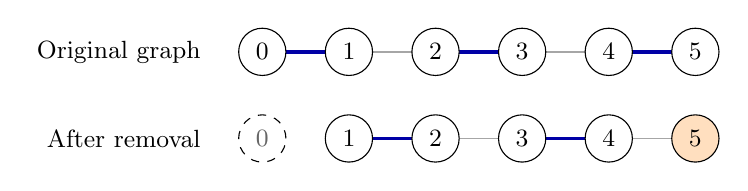
\begin{tikzpicture}[
  x=11mm,y=11mm,font=\small,
  vertex/.style={circle,draw,fill=white,minimum size=6mm,inner sep=1pt},
  path edge/.style={draw=black!35,semithick},
  pair edge/.style={draw=blue!65!black,line width=1.4pt}
]
\node[anchor=east] at (-0.6,0) {Original graph};
\node[anchor=east] at (-0.6,-1) {After removal};
\foreach \row in {0,-1} {
  \foreach \i in {1,...,4} {
    \draw[path edge] (\i,\row) -- ++(1,0);
  }
}
\draw[pair edge] (0,0) -- (1,0);
\draw[pair edge] (2,0) -- (3,0);
\draw[pair edge] (4,0) -- (5,0);
\draw[pair edge] (1,-1) -- (2,-1);
\draw[pair edge] (3,-1) -- (4,-1);
\foreach \i in {0,...,5} {
  \node[vertex] at (\i,0) {\i};
}
\node[vertex,dashed,text=black!60] at (0,-1) {0};
\foreach \i in {1,...,4} {
  \node[vertex] at (\i,-1) {\i};
}
\node[vertex,fill=orange!25] at (5,-1) {5};
\end{tikzpicture}
